\section{Overview of Code}

\subsection{Source Code}
The code for this project and related documentation can be found in the repository below on the master branch.
\bigskip

\noindent
\textbf{Link:} https://github.com/rohitmukherjee/High-Performance-DSLs

\subsection{Functional/Performance DSL Code Base}
An overview of the convenience methods/types exposed in the Scala DSL and the API of the Python system are shown below. Private and Protected members have not been shown and test packages/code have been excluded from the section in the interest of brevity.
\bigskip

\noindent
A diagram of the Scala code base is shown below. Scala does not have tooling support for UML generation but allows diagrams like the one below to be generated. The shapes in \textbf{green} represent \textbf{types}, \textbf{orange} represents composite pattern usage or \textbf{client relationships} and \textbf{pink} represents \textbf{inheritance}.

\begin{figure}[H]
  \centering
    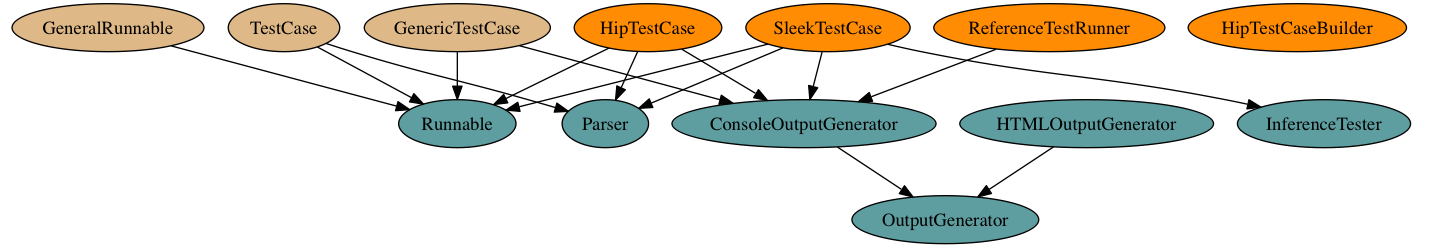
\includegraphics[height=80px]{figures/scala_uml.png}
  \caption{Overview of first DSL}
\end{figure}

\noindent
The exposed APIs and client facing DSL types are briefly explained below:

\begin{itemize}
\item package systemTestingDSL
    \begin{itemize}
        \item \textbf{Object FileSystemUtilities} - Object with utility file system manipulation methods
        \item \textbf{Trait Runnable} - Models behaviour of any executable/command that can be run
        \item \textbf{Case Class General Runnable} - Models implementation of any executable/command 
        \item \textbf{Case Generic Test Case} - Test Case for any generic purpose runnable
        \item \textbf{Case Class HipTestCase} - Test Case especially for Hip verification
        \item \textbf{Object HipTestCaseUsage} - Client with hip test cases
        \item \textbf{Object HipTestSuiteUsage} - Client with hip test suites
        \item \textbf{Object SleekTestSuiteUsage} - Client with sleek test suites
        \item \textbf{Object SleekTestCaseUsage} - Client with sleek test cases
        \item \textbf{Object InferenceDefaults} - Sensible defaults for inference checking
        \item \textbf{Trait InferenceTester} - Trait with functionality to verify (a,b) tuples
        \item \textbf{Object Main} - This is passed arguments by sbt and contains factory methods
        \item \textbf{Trait Parser} - Regex and rule based parser methods are described here
        \item \textbf{Class ReferenceTestRunner} - Runs regression tests
        \item \textbf{Class RegressionTestReferenceBuilder} - Constructs regression tests
        \item \textbf{Case Class SleekTestCase} - Test Case especially for Sleek verification
        \item \textbf{Case Class TestCase} - Any Test Case
        \item \textbf{Case Class GenericTestSuite} - Automated testing of files of a certain type found          using regex matching
        
    \end{itemize}
\item package systemTestingDSL.outputGenerator
    \begin{itemize}
        \item \textbf{Trait OutputGenerator} - Specifies contract for output generation including logging, error, expected and success
        \item \textbf{Trait ConsoleOutputGenerator} - Mixin with methods which implement OutputGenerator's methods for console output
        \item \textbf{Trait HTMLOutputGenerator} - Mixin with methods which implement OutputGenerator's methods for HTML output
    \end{itemize}
\item package systemTestingDSL.matchers
    \begin{itemize}
    \item \textbf{Trait Matcher} - Models behaviour for any generic matcher
    \item \textbf{DiffMatcher} - Matches two files based on their diff
    \end{itemize}
\item package systemTestingDSL.testSuite
    \begin{itemize}
    \item \textbf{Case Class HipTestSuite} - Suite of hip test cases
    \item \textbf{Case Class SleekTestSuite} - Suite of sleek test cases
    \end{itemize}
\end{itemize}

\subsection{Reporting DSL Code Base}
The Reporting DSL was implemented both in Python and Scala for comparison purposes. The code bases of both The Python version and Scala version ar documented below.

\subsubsection{Python DSL Version}
Diagrams of the Python code base is shown below. The first diagram captures the UML of the system and only shows portion of the code (parts that are object oriented). The second shows the \textbf{package diagram} with dependency information. The reason they are different is because a part of the tool is written in scripting style and the remaining in object oriented style. This also adequately reflects the versatility of a dynamic language such as Python.

\begin{figure}[H]
  \centering
    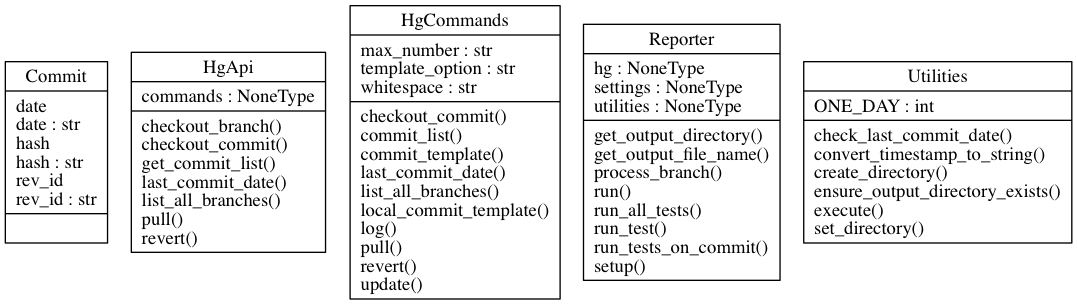
\includegraphics[height=130px]{figures/python_dsl_classes.png}
  \caption{UML diagram}
\end{figure}

\noindent
An API for the Distributed Version Control System (DVCS) Mercurial, had to be written because the Mercurial team stated that their current API is being overhauled. The API developed implements a subset of the full command set based on usage. It is written as a wrapper around terminal commands.

\begin{figure}[H]
  \centering
    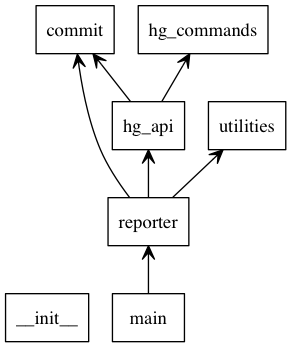
\includegraphics[height=150px]{figures/python_dsl_package.png}
  \caption{Package diagram}
\end{figure}

\subsubsection{Scala DSL Version}

The reporting DSL was also developed in Scala. The UML followed is identical to the one followed for the Python version. The screenshot below shows the declarative syntax developed for the DSL.

\begin{figure}[H]
  \centering
    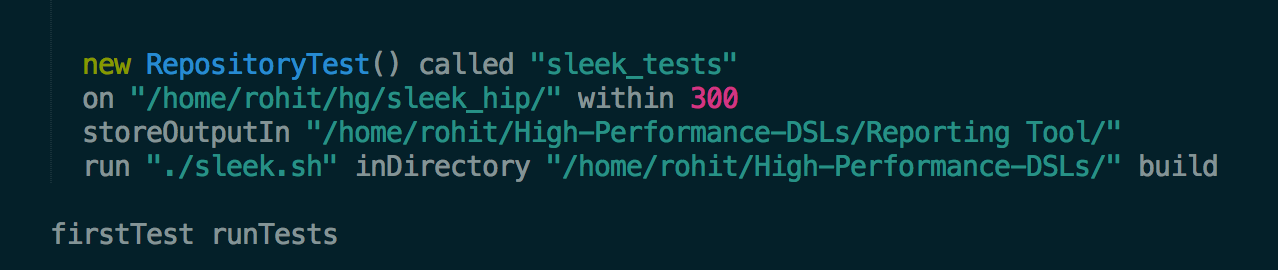
\includegraphics[height=100px]{figures/reportingDSL.png}
  \caption{Scala DSL syntax}
\end{figure}
 
\noindent
The exposed APIs and client facing DSL types are briefly explained below:

\begin{itemize}
\item package repositoryTestingDSL
    \begin{itemize}
        \item \textbf{Case Class Commit} - Models implementation of a version control commit
        \item \textbf{Trait Execute} - Trait represents any class that has an operating system call being made
        \item \textbf{Object HgApi} - Provides access to mercurial methods
        \item \textbf{Object HgCommands} - Model representing the commands recognized by mercurial.
        \item \textbf{Object Utilities} File system utility methods
        \item \textbf{Class RepositoryTest} - Represents a single Repository Test
\end{itemize}
\end{itemize}

\newpage